%%
%% Template Experiments.tex
%%

\chapter{Experiments}
\label{cha:Experiments}

In this chapter, we follow our previous approach
in~\cite{gouldlearning} and conduct two experiments with
different purposes. We first examine our method's effectiveness
by comparing our results with~\cite{gouldlearning,Gould:ICML2011}
on a synthetic checkerboard. We then extend our work to the
real-world ``GrabCut'' problem introduced in
section~\ref{sec:grabcut} and comparing our result with previous
researches \cite{Rother:SIGGRAPH04} to investigate
our new methods' performance.

\section{Synthetic Checkerboard}
\label{sec:synth-check}

Since the main contribution of our work is extending our previous
approximate formulation of lower linear envelope potentials to an
exactly formulation, it is necessary to compare the results on
synthetic checkerboard to previous work~\cite{gouldlearning}.

In this section we will experiment our method on three different
problem instances: checkerboard with squares containing
monotonous color~\ref{sec:monot-color-squar}, checkerboard with
squares containing more pixels of one color over
another~\ref{sec:unbal-color-squar} and checkerboard with
uniformly colored squares containing unbalanced
color~\ref{sec:unif-distr-squar}.

\subsection{Experiment Settings}
\label{sec:experiment-settings}

An image of synthetic checkerboard contains $8 \times 8$ pixel
squares. Each square (clique) contains $16 \times 16$ (256)
pixels. The color of each pixel is either black $0$ or white $1$.
Given a ground-truth checkerboard image
$\by^*=y^*_1,\dots,y^*_{16384}$, the observed unary terms
$\by=y_1,\dots,y_{16384}$ are generated as followings. Let
$\eta_0$ and $\eta_1$ be the signal-to-noise ratios for the black
and white squares, the unary terms are generated by destroying
groud-truth label to noisy input
\begin{align}
  \label{eq:noisy_checkerboard}
  y_i = \eta_0 \ind{y^\star_i = 0} - \eta_1 \ind{y^\star_i = 1} + \delta_i
\end{align}
where $\delta_i
\sim \U(-1, 1)$ is additive i.i.d.\ uniform noise. $\ind{x}$ is
an indicator function which equals $1$ when $x$ is true and $0$
otherwise. The task is to recover the ground-truth checkerboard
from the noisy input.

Our MRF is constructed on this image by associating each node in
the MRF to each pixel in the image. Thus our MRF contains $8
\times 8 \times 256 = 16,384$ variables. The energy function used
in this experiment follows equation~\eqref{eq:energyfunction_UPH}
without pairwise terms.

\begin{align}
  \label{eq:syncheck_energy}
  E(\by;\btheta)=\theta^U\sum_{i\in \N}{\phi^U(\by_i)}+
  \sum_{\by_c\in \C}{\phi^H(\by_c,\bz_c;\btheta^H)}
\end{align}
where $\phi^U(\by_i)=\by_i$ and $\theta^U$ is a scalar weight for
unary terms. $\phi^H(\by_c,\bz_c;\btheta^H)=\btheta^{H\;T} \!
\phi(\by_c,\bz_c)$ is equivalent to
equation~\eqref{eq:llsvm_innerprod_energy} and added for each
square (clique $c$) in the checkerboard. The number of linear
equations $K$ in equation~\eqref{eq:llsvm_param} is set to be
$10$. The parameters $\theta^U$ and $\btheta^H$ are learned using
\algref{alg:learning} with $MaxIter=100$. 

\subsection{Monotonous Colored Squares}
\label{sec:monot-color-squar}

\begin{figure}[hb]
  \centering
  \setlength{\tabcolsep}{2pt}
  \begin{tabular}{cc}
    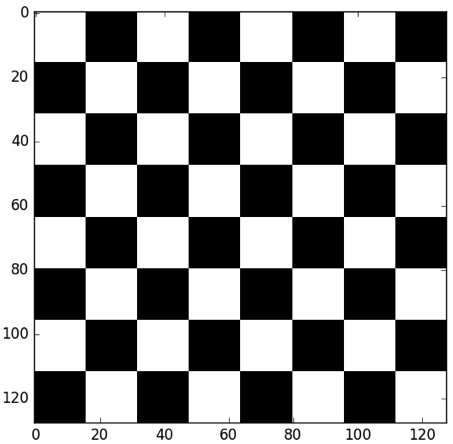
\includegraphics[width=0.5\columnwidth]{Experiments/figures/mono_gt.png}&
                                                                            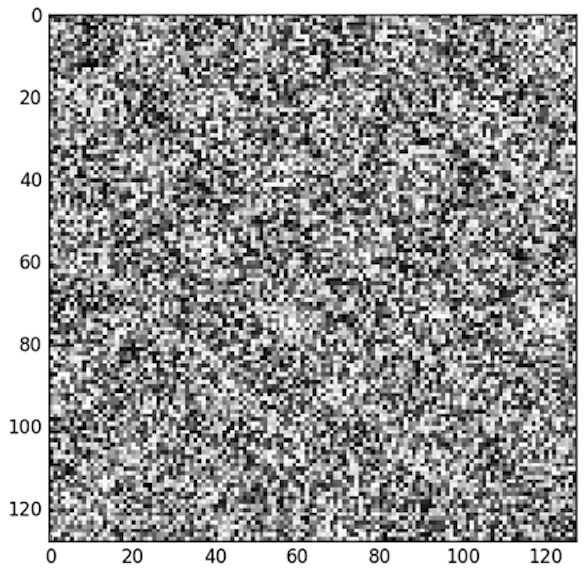
\includegraphics[width=0.5\columnwidth]{Experiments/figures/mono_noisy.png}\\
    {\small (a)} & {\small (b)} 
  \end{tabular}
  \caption{\label{fig:mono_checkerboard} Example for monotonous
    colored squares. figure (a) is the ground-truth checkerboard.
    Figure (b) is the noisy input (unary terms) destroyed by
    equation~\eqref{eq:noisy_checkerboard}}
\end{figure}

We first repeat our previous black and white checkerboard
experiment~\cite{Gould:ICML2011,gouldlearning} in order to
examine the correctness of our new formulation. Each clique
(square) $c\in \C$ in the checkerboard contains either all white
pixels $y_i=1 ,\;\forall i \in c$ or all black pixels $y_i=0
,\;\forall i \in c$. Figure~\ref{fig:mono_checkerboard}
illustrates the ground-truth checkerboard and the noisy input
destroyed by equation~\eqref{eq:noisy_checkerboard} with
$\eta_0=\eta_1=0.1$. Figure~\ref{fig:mono_results} shows the
results of our new method (on the bottom) together with our
previous method~\cite{gouldlearning} (on the top).

\begin{figure}[ht]
  \centering
  \setlength{\tabcolsep}{2pt}
  \begin{tabular}{cc}
    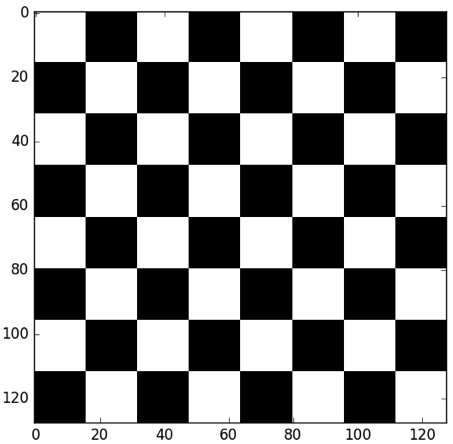
\includegraphics[width=0.3\columnwidth]{Experiments/figures/mono_gt.png}&
                                                                              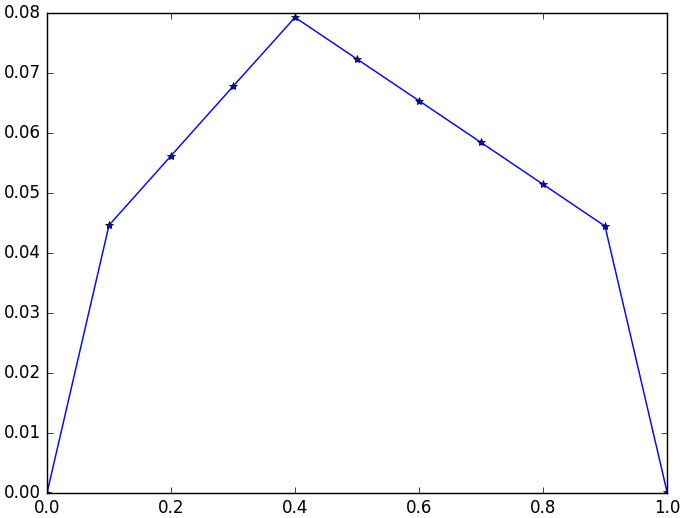
\includegraphics[width=0.4\columnwidth]{Experiments/figures/mono_old.png}\\
    {\small (a)} & {\small (b)} \\
    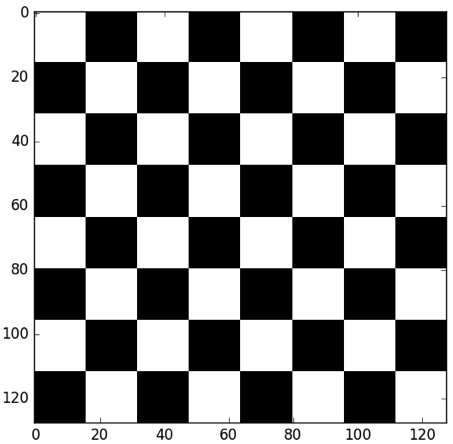
\includegraphics[width=0.3\columnwidth]{Experiments/figures/mono_gt.png}&
                                                                              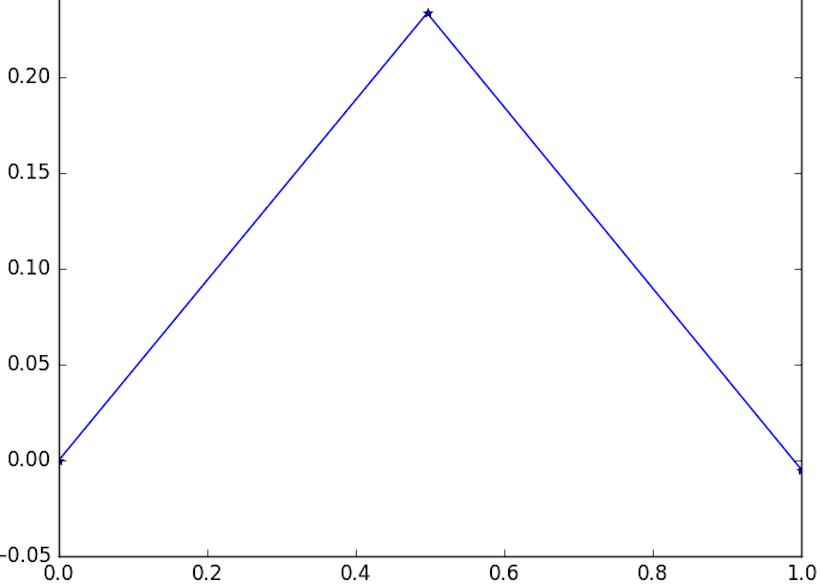
\includegraphics[width=0.4\columnwidth]{Experiments/figures/mono_new.png}\\
    {\small (c)} & {\small (d)} 
  \end{tabular}
  \caption{\label{fig:mono_results} Results comparison for
    monotonous colored squares. Figure (a) and Figure (c) are
    inferred checkerboard from our previous and current
    formulation separately. Figure (b) and Figure (d) are lower
    linear envelopes learned by each formulation.}
\end{figure}

From figure~\ref{fig:mono_results} we conclude that both
formulations can recover checkerboard perfectly so our new
formulation's accuracy is as good as previous one. However,
there are significant differences between structural SVM
formulation (previous method) and latent structural SVM
formulation. There are $10$ active linear functions in
figure~\ref{fig:mono_results} (b) while there are only $2$ active
linear functions in figure~\ref{fig:mono_results} (d). Shapes
learned by each formulation are also significantly different.

In general, the second result is more preferable than the first
one. The reason is despite the image contains 64 cliques, there
are only two kinds of squares in the image: completely black and
completely white. Accordingly, our model only see two kinds of
cliques: completely $0$s (black) and completely $1$s (white). In
this case, a lower linear envelope contains two linear functions
is enough for encoding consistency information. This is reflected
in figure~\ref{fig:mono_results} (d) which gives least penalty
(0) when the clique value $W_C(y_c)$ equals either $0$ or $1$. It
gives the highest penalty when $W_C(y_c)$ is in the middle
because our model has least probability seen that in training
data. The results certificates that our latent structural SVM
formulation can learn lower linear envelope exactly. Therefore,
we say that our new method learns more preferable lower linear
envelope.

In terms of computational performance, because our initial point
are generated randomly using \algref{alg:init_theta}, the
performance various between runnings. On average it takes 2
\emph{outer loops} and 47 \emph{inner loops} to converge. Which
means the latent structural SVM formulation spends $3.5$ times
iterations to converge than previous one ($27$ iterations).
Each \emph{inner loop} took under 1s with inference taking about
120ms on a $2.7$GHz dual-core Intel CPU, which is the same as our
previous method.



\subsection{Unbalanced Colored Squares}
\label{sec:unbal-color-squar}

Experiment in section~\ref{sec:monot-color-squar} proves that our
latent structural SVM formulation can learn the lower linear
envelope exactly. In this section we conduct further experiment
to investigate its capability of representing unbalanced input.
The desirable result of this experiment should be the shape of
the lower linear envelope shifting along with the changing of
input data.

We design our checkerboards contain unbalanced colored squares as
shown in figure~\ref{fig:unba_checkerboard}.

\begin{figure}[hb]
  \centering
  \setlength{\tabcolsep}{2pt}
  \begin{tabular}{cc}
    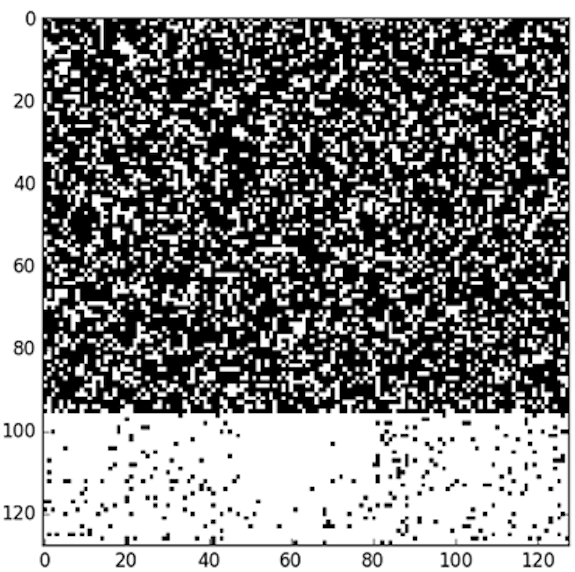
\includegraphics[width=0.5\columnwidth]{Experiments/figures/unba_black.png}&
                                                                            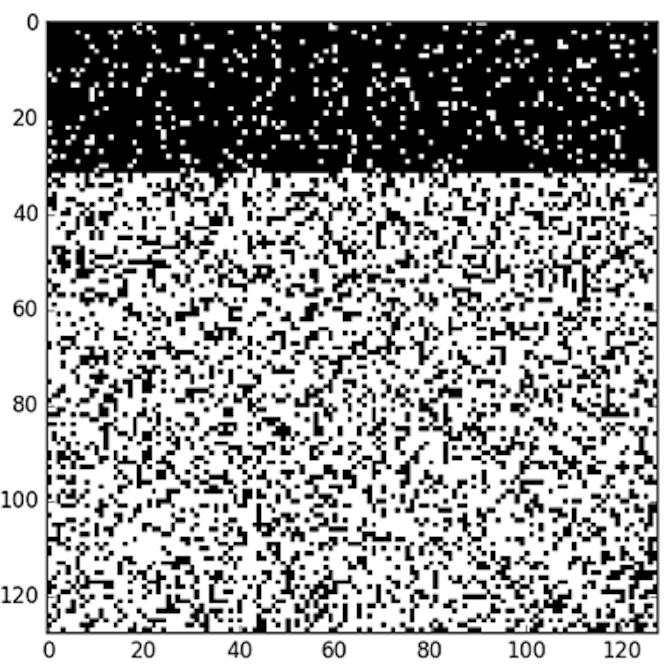
\includegraphics[width=0.5\columnwidth]{Experiments/figures/unba_white.png}\\
    {\small (a)} & {\small (b)} 
  \end{tabular}
  \caption{\label{fig:unba_checkerboard} Example for unbalanced
    colored squares. In figure (a) $75\%$ cliques contain more
    than $85\%$ black pixels while $25\%$ cliques contain more
    than $85\%$ white pixels. Figure (b) is the opposite of
    figure (a)}
\end{figure}

As before, figure~\ref{fig:unba_results} shows results learned by
structural SVM (top row) and latent structural SVM (bottom row).
The accuracy performance of both methods are almost the same.
Both methods are able to recover $45\%-50\%$ pixels. The shape of
each formulations' results are both preferable and very similar
when compared to each other. The most significant difference is
the number of linear functions (10 active linear functions v.s.
2). In terms of computational performance, our previous method
only takes $10$ iterations to converge while the latent
structural SVM formulation takes $89$ iterations. Our new method
is much more computational expensive than our previous method.

\begin{figure}[ht]
  \centering
  \setlength{\tabcolsep}{2pt}
  \begin{tabular}{cc}
    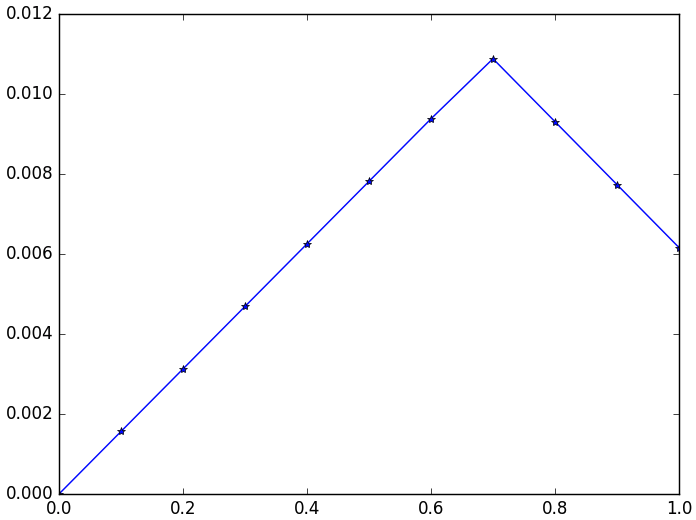
\includegraphics[width=0.5\columnwidth]{Experiments/figures/unba_black_res_old.png}&
                                                                              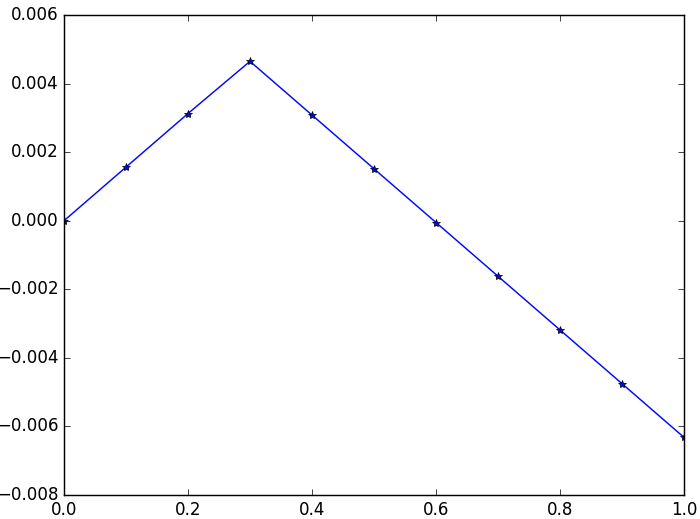
\includegraphics[width=0.5\columnwidth]{Experiments/figures/unba_white_res_old.png}\\
    {\small (a)} & {\small (b)} \\
    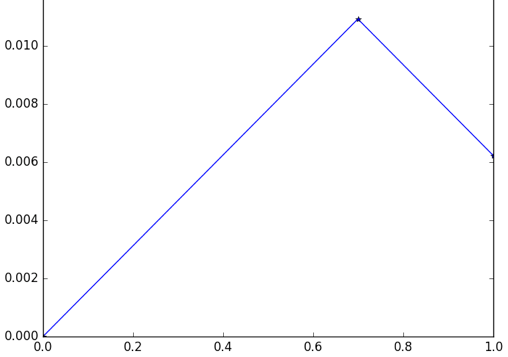
\includegraphics[width=0.5\columnwidth]{Experiments/figures/unba_black_res_new.png}&
                                                                              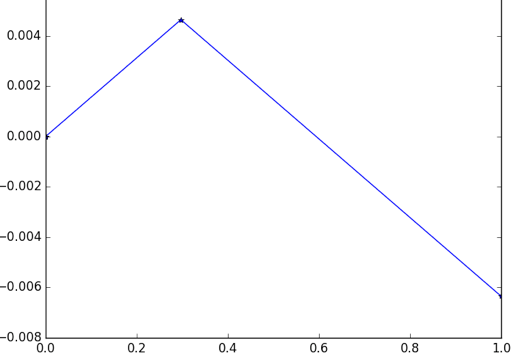
\includegraphics[width=0.5\columnwidth]{Experiments/figures/unba_white_res_new.png}\\
    {\small (c)} & {\small (d)} 
  \end{tabular}
  \caption{\label{fig:unba_results} Results comparison for
    unbalanced colored squares. Figure (a) and Figure (b) are
    lower linear (more black and more white) envelopes learned by
    structural SVM. Figure (c) and Figure (d) are learned by
    latent structural SVM.}
\end{figure}

\bigskip
\bigskip
\bigskip
\bigskip
\bigskip
\bigskip

\subsection{Uniformly Colored Squares}
\label{sec:unif-distr-squar}

All of the above experiments show that our new method can
significantly simplify the shape of the lower linear envelope
function while maintaining the inference performance at the same
level. However, one significant cost is the computational
performance. It still remains obscure if there exists any other
advantages. In this section we design a much harder problem.
$W_c(y_c)$ is uniformly distributed from $0$ to $1$.
Figure~\ref{fig:ba_gt} shows the result. The preferable shape of
the lower linear envelope should contain a line which is parallel
to the x-axis.

\begin{figure}[t]
  \centering
  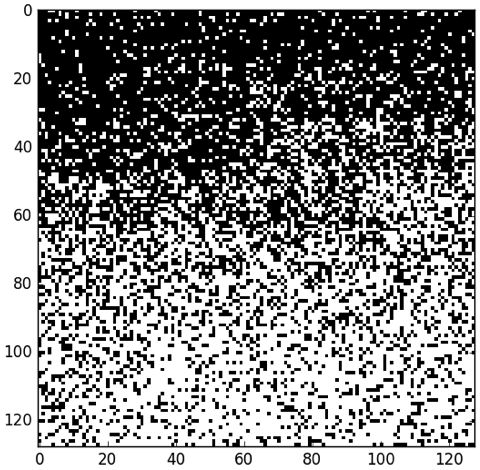
\includegraphics[width=0.5\columnwidth]{Experiments/figures/ba_gt.png}
  \caption{\label{fig:ba_gt} Uniformly colored squares example.
    $W_{\!c}(\by_c) = \sum_{i \in c} w^c_i y_i$ is uniformly
    distributed from $0$ to $1$.}
\end{figure}

Results are shown in figure~\ref{fig:ba_res}. As we can see
that shapes are very different between two formulations. Our
latent structural formulation (figure~\ref{fig:ba_res} (b))
learned a very flat representation of the lower linear envelope
function, which is much preferable, while the structural SVM
formulation preserves much concavity in the shape. This might
because in previous work~\cite{gouldlearning,Gould:ICML2011}
we imposed strict concave constraints on parameter vector
$\btheta$.

The performance of accuracy also various significantly. Under
this formulation our new method is still able to recover
$45\%-50\%$ pixels while our previous can only recover
$25\%-30\%$ pixels on average. Therefore, our new formulation
finally outperforms previous one. In terms of computational
performance, the new formulation takes $129$ \emph{inner loops}
in total (2 \emph{outer loops}) while our previous formulation
takes $75$ iterations to converge. Although the new formulation
is still more computational expensive than previous one, the gap
decreases significantly.

We consider all of those improvements are due to our new method
is able to learn the lower linear envelope exactly.

One subtle thing is that the linear function on the right side in
figure~\ref{fig:ba_res} (b) decreases sharply which seems
abnormally at first glance. The reason is that we assume $b_1=0$
in section~\ref{sec:llep} which fixes the y-intercept of the
first linear function to be zero. Therefore the last linear
function can be arbitrarily deep while the first linear function
is fixed at the original point.

\clearpage

\begin{figure}[ht]
  \centering
  \setlength{\tabcolsep}{2pt}
  \begin{tabular}{cc}
    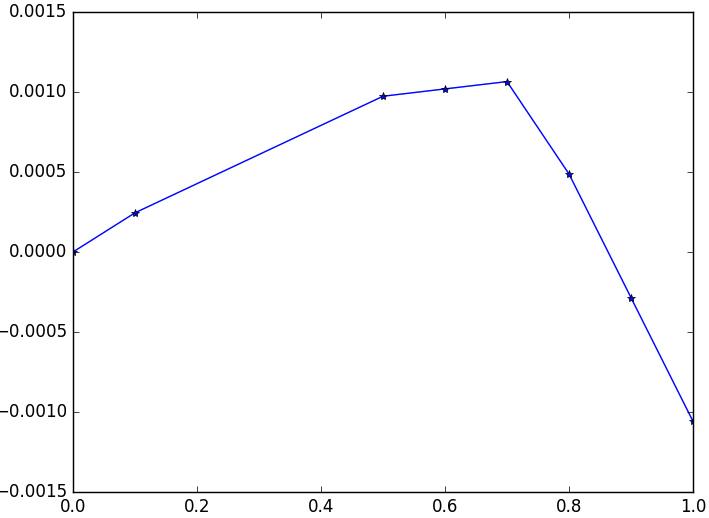
\includegraphics[width=0.5\columnwidth]{Experiments/figures/ba_res_old.png}&
                                                                            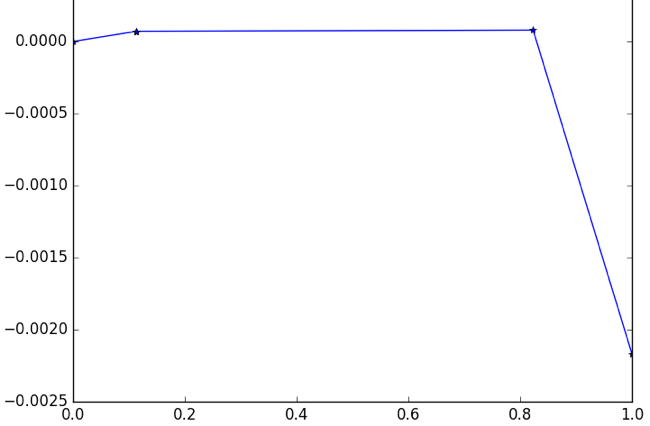
\includegraphics[width=0.55\columnwidth]{Experiments/figures/ba_res_new.png}\\
    {\small (a)} & {\small (b)} 
  \end{tabular}
  \caption{\label{fig:ba_res} Results of uniformly colored
    squares experiment. Figure (a) is the result learned by
    structural SVM formulation. Figure (b) is the result learned
    by latent structural SVM formulation.}
\end{figure}

\subsection{Conclusions}
\label{sec:synth-check-conc}

From above experiments we conclude our findings as followings:

\begin{itemize}
\item All of those experiments verified that our latent
  structural formulation is able learn the lower linear envelope
  exactly.
\item In general (see section~\ref{sec:monot-color-squar} and
  section~\ref{sec:unbal-color-squar}), our new method have
  equivalent accuracy performance to our old method (structural
  SVM formulation\cite{Gould:ICML2011,gouldlearning}).
\item In terms of computational performance, the new formulation
  is much more computational expensive than the previous one
  during training. However, it is more efficient during testing
  due to it simplicity for the lower linear envelope potentials.
\item For harder problem (see
  section~\ref{sec:unif-distr-squar}), the new method outperforms
  the previous one significantly. The gap of computational
  performance also decreases a significant amount.
\end{itemize}

\clearpage

\section{Foreground Extraction}
\label{sec:foregr-extr}

To evaluate our method on real-world applications, we repeat the
``Interactive Figure-Ground Segmentation'' experiment in our
previous researches~\cite{gouldlearning,Gould:ICML2011}. As
described in section~\ref{sec:grabcut}, the goal of this
experiment is to extract foreground pixels from a bounding box of
the object. We follow settings in previous work and replace
the max margin algorithm with latent structural SVM
\algref{alg:learning}.

\subsection{Experiment Settings}
\label{sec:experiment-settings-grabcut}

The data set we use is collected by~\citename{Lempitsky:ICCV09}
which contains $50$ images (contains $630\times480$ pixels on
average) with ground-truth labels and user-annotated bounding
boxes. Following previous work we perform
\algref{alg:learning} by leave-one-out cross-validation on this
data set. In order to be comparable with previous results, the
performance is measured by \emph{accuracy}. Our energy function
for this problem is defined as:

\begin{align}
  \label{eq:grabcut_mrflssvm_energy}
  E(\by;\btheta)=\theta^U\sum_{i\in \N}{\phi^U(\by_i)}+
  \theta^P\sum_{(i,j)\in \E}{\phi^P(\by_i,\by_j)}+
  \sum_{\by_c\in \C}{\phi^H(\by_c,\bz_c;\btheta^H)}
\end{align}

As we described in section~\ref{sec:grabcut}, unary terms are
generated by GMMs (both foreground and background) trained by
\emph{GrabCut}~\cite{Rother:SIGGRAPH04} algorithm. The unary
terms are assigned as following:

\begin{table}[h]
  \normalsize
  \centering
  \begin{tabular}{|l|c|c|}
    \hline
    {\sc Unary} & {\sc $0$} & {\sc $1$}\\
    \hline
    $\phi^U(y_i)$ & $\phi^U(0,\bk_i,\btheta,\bz_i)$ & $\phi^U(1,\bk_i,\btheta,\bz_i)$ \\
    \hline
  \end{tabular}
  \caption{\label{tab:grabCut_unary} Table of GrabCut unary
    terms. $\phi^U$ is taken from
    equation~\eqref{eq:grabcut_energy}. $1$ is the label for
    foreground and $0$ for background}
\end{table}

The pairwise terms are defined as:
\begin{align}
  \label{eq:mrflssvm_grabcut_pairwise}
  \phi^P(\by_i,\by_j) = \frac{\lambda}{d_{ij}}[[y_i\neq y_j]]exp\bigg\{-\frac{||x_i-x_j||^2}{2\beta}\bigg\} \text{~,~for~~} \forall (i,j)\in \E
\end{align}

where $\E$ denotes the set of pairs of neighboring pixels which
is defined as 8-way adjacent pixels (horizontally, vertically and
diagonally). $d_{ij}$ is the Euclidean distance of neighboring
pixels. $x_i$ is the RGB value vector. $\beta$ denotes the
expectation over $(x_i-x_j)^2$. The only free parameter $\lambda$
is learned by \algref{alg:learning} during cross-validation and
determines the strength of the pairwise smoothness term.

The \emph{SLIC} algorithm introduced in
section~\ref{sec:superpixel} is used to generate cliques $c\in\C$
for higher order terms.
$\phi^H(\by_c,\bz_c;\btheta^H)=\btheta^{H\;T} \!
\phi(\by_c,\bz_c)$ is equivalent to
equation~\eqref{eq:llsvm_innerprod_energy} and added for each
clique $c$ in the image. The number of linear equations $K$ in
equation~\eqref{eq:llsvm_param} is set to be $10$.

Then we run the \algref{alg:learning} with $MaxIter=100$. Results
are shown in section~\ref{sec:grabcut_exp_result}. 

\subsection{Experiment Result}
\label{sec:grabcut_exp_result}

In this section we compare our new latent structural SVM
formulation's results with our previous
work~\cite{gouldlearning}. On average it takes $5.3$ hours to
train a cross-validation fold while our previous method only
takes $3$ hours. For some folds our method can take more than $8$
hours and still not converge. Table~\ref{tab:grabCut_acc} shows
comparison between different models:

\begin{table}[h]
  \normalsize
  \centering
  \begin{tabular}{|l|c|}
    \hline
    {\sc Model} & {\sc Accuracy}\\
    \hline
    Baseline & 90.9 \\
    \hline
    Structural SVM Formulation & 91.6 \\
    Latent SSVM Formulation & 92.27 \\
    \hline
  \end{tabular}
  \caption{\label{tab:grabCut_acc} GrabCut experiment results
    comparison. Data of Baseline model and Structural SVM model
    is from previous work~\cite{gouldlearning}.}
\end{table}

It turns out that our new formulation slightly outperforms our
previous method by $0.6\%$. The following
table~\ref{tab:grabCut_hist} shows a more detailed accuracy
distribution among $50$ images:

\begin{table}[h]
  \normalsize
  \centering
  \begin{tabular}{|l|c|}
    \hline
    {\sc Accuracy Interval} & {\sc Number of images}\\
    \hline
    Over $99.5\%$ & $35$ \\
    \hline
    $90\%-99.5\%$ & $9$ \\
    \hline
    $70\%-90\%$ & $4$ \\
    \hline
    $50\%-70\%$ & $1$ \\
    \hline
    Below $50\%$ & $1$ \\
    \hline
  \end{tabular}
  \caption{\label{tab:grabCut_hist} GrabCut results' accuracy
    distribution.}
\end{table}

From this table we can conclude that our new formulation performs
very well on $75\%$ of images in the data set. From
figure~\ref{fig:flower_results} to
figure~\ref{fig:portrait_results} show the comparison of results
which we illustrated in previous work~\cite{gouldlearning}.
Figure in the middle column is the ground-truth foreground image.
Figure on the left is the foreground inferred by our previous
method. Figure on the right is inferred by our new method.

% grabcut results

\begin{figure}[ht]
  \begin{center} \setlength{\tabcolsep}{0pt}
    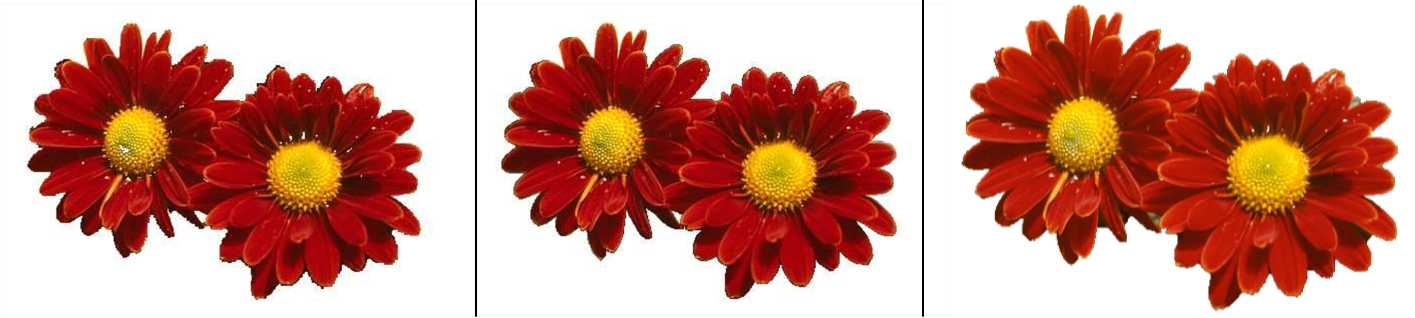
\includegraphics[width=\linewidth]{Experiments/figures/124080.png}
\\
  \caption{\label{fig:flower_results}GrabCut Results.}
  \end{center}
\end{figure}

\begin{figure}[ht]
  \begin{center} \setlength{\tabcolsep}{0pt}
    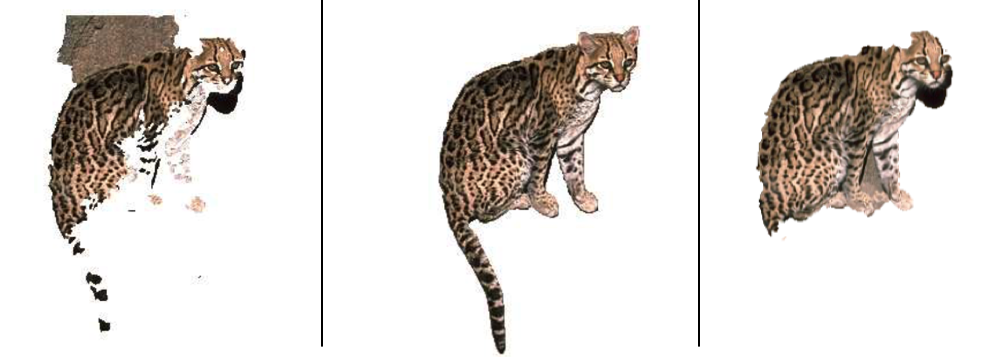
\includegraphics[width=\linewidth]{Experiments/figures/326038.png}
\\
  \caption{\label{fig:cheetah_results}GrabCut Results.}
  \end{center}
\end{figure}

\begin{figure}[ht]
  \begin{center} \setlength{\tabcolsep}{0pt}
    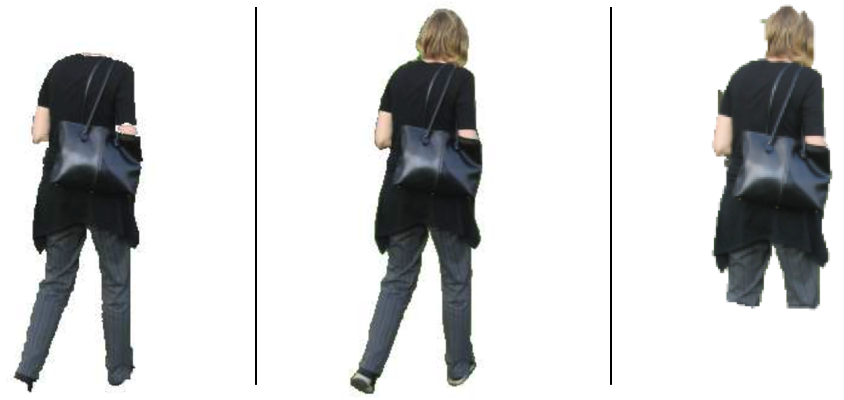
\includegraphics[width=\linewidth]{Experiments/figures/person5.png}\\
  \caption{\label{fig:person_results}GrabCut Results.}
  \end{center}
\end{figure}

In figure~\ref{fig:flower_results}, our new method has a very
strong results. It almost perfectly extracted the foreground
image. The accuracy is over $99.5\%$. In
figure~\ref{fig:cheetah_results} our new method still performs
better. However, it left the cheetah's tail out compared to our
previous method. One important thing to notice is that there are
many holes in the image on the left (inferred by our previous
method) while the image inferred by our new method is very smooth
without holes. This certificates that by learning the lower
linear envelope exactly, our new method has a better performance
on preserving higher order consistency. In
figure~\ref{fig:person_results} two methods have almost the same
performance. Previous method left the woman's head but was
able to capture her full legs while our new method only able to
capture half of her legs but with full head.

\bigskip
\bigskip
\bigskip
\bigskip

However, the performance various significantly between images. In
figure~\ref{fig:portrait_results}, even though the sculpture
inferred by our new method is still very smooth without any hole
on it, our method failed to segment the background out of the
foreground (there are large amount of pixels belong to stairs and
glass). Our model completely fails to learn the image
``189080.png'' which has the worst performance $42.5\%$ (the
\algref{alg:learning} stopped at the maximum number of iterations
which is 10 \emph{outer loops} and 100 \emph{inner loops} for
each \emph{outer loop}). The inferred foreground image is
completely blank as shown in figure~\ref{fig:grabcut_worst}.


\begin{figure}[t]
  \begin{center} \setlength{\tabcolsep}{0pt}
    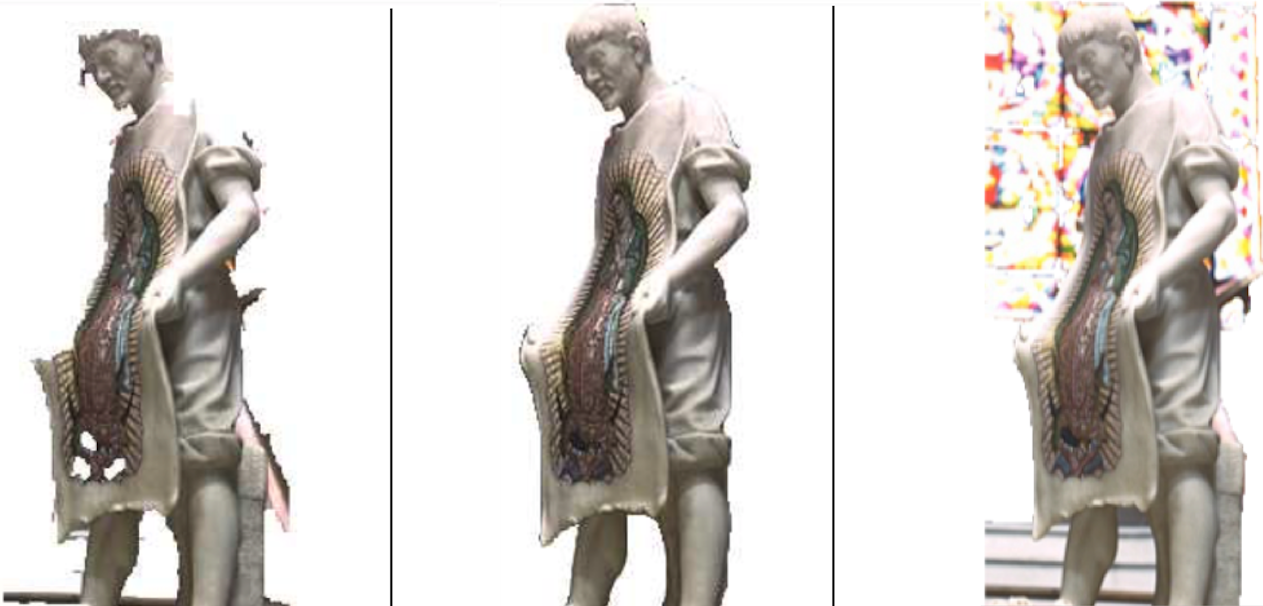
\includegraphics[width=\linewidth]{Experiments/figures/24077.png}\\
  \caption{\label{fig:portrait_results} GrabCut Results.}
  \end{center}
\end{figure}

\begin{figure}[t]
  \begin{center} \setlength{\tabcolsep}{0pt}
    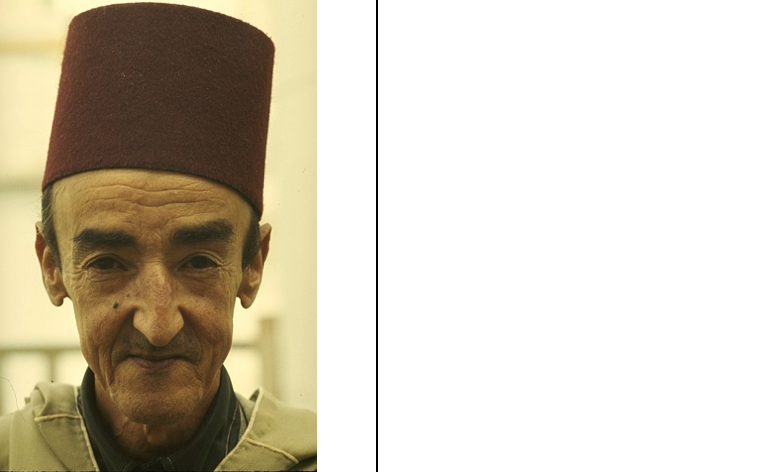
\includegraphics[width=0.5\linewidth]{Experiments/figures/189080.png}
\\
\caption{\label{fig:grabcut_worst} Worst accuracy image. The
  accuracy is only $42.5\%$. The foreground inferred is
  completely blank which means information learned by our model
  is failed to be generalize to this image.}
  \end{center}
\end{figure}

\clearpage

\subsection{Conclusions}
\label{sec:grabcut-conc}

From above experiments we conclude our findings as followings:

\begin{itemize}
\item In general, our new method outperforms previous one.
  The accuracy is increased by $0.6\%$. This might because our
  new method learns the lower linear envelope exactly thus has a
  richer representation than previous one.
\item In general, our new method has a better higher-order
  consistency. This can be seen from
  figure~\ref{fig:flower_results} to
  figure~\ref{fig:portrait_results}. This is also because the
  lower linear envelope function has better quality than our
  previous method.
\item The new method's performance various differently among
  images. The performance ranges from $42.5\%$ to $99.5\%$.
\item The new method is more computationally expensive than our
  previous method during training. It takes $5.3$ hours to train
  one cross-validation fold while previous method only takes
  $3$ hours. However, it is more efficient during testing due to
  it simplicity for the lower linear envelope potentials.
\item There seems like to exist some generalization issues in our
  \algref{alg:learning}. For example, the new method has bad
  performance of filtering background in
  figure~\ref{fig:portrait_results} and it completely fails to
  infer the figure~\ref{fig:grabcut_worst}.
\end{itemize}



\clearpage
\cleardoublepage



%%% Local Variables:
%%% mode: latex
%%% TeX-master: "../thesis"
%%% End:
